\documentclass[aps,pra,reprint,superscriptaddress,nofootinbib]{revtex4-2}

\usepackage{amsmath,amssymb,amsfonts}
\usepackage{graphicx}
\usepackage{xcolor}
\usepackage{bm}
\usepackage{algorithm}
\usepackage{algpseudocode}
\usepackage{booktabs}
\usepackage{tikz}
\usepackage{pgfplots}
\pgfplotsset{compat=1.18}
\usetikzlibrary{shapes,arrows,positioning,calc}
\usepackage{hyperref}
\hypersetup{
    colorlinks = true,
    linkcolor  = blue,
    citecolor  = blue,
    urlcolor   = blue
}

% Custom commands
\newcommand{\R}{\mathbb{R}}
\newcommand{\E}{\mathbb{E}}
\newcommand{\M}{\mathcal{M}}
\newcommand{\N}{\mathcal{N}}
\newcommand{\C}{\mathcal{C}}
\newcommand{\A}{\mathcal{A}}
\newcommand{\D}{\mathcal{D}}
\newcommand{\T}{\mathcal{T}}
\newcommand{\zctx}{z_{\mathrm{ctx}}}
\newcommand{\sNEP}{s_{\mathrm{NEP}}}

\begin{document}

\title{ALFM: Adaptive Latent Feedback Model for Institutional Memory in Foundation Model Deployments}

\author{David Ahmann}
\affiliation{Independent Researcher, Toronto, Canada}

\date{\today}

\begin{abstract}
Foundation models are pretrained once and deployed frozen, creating three fundamental gaps in enterprise AI systems: no memory of past failures, no calibrated self-doubt, and no safe mechanism for continual learning from corrections. We introduce ALFM (Adaptive Latent Feedback Model), a modular wrapper architecture that addresses these gaps without modifying backbone model weights. ALFM consists of three novel components: (1) the Negative Evidence Prior (NEP), a tenant-isolated vector memory that stores failure patterns and provides risk signals at inference time; (2) the Consensus Engine, a multi-agent system that arbitrates between semantic intuition and heuristic rules to decide when to trust, abstain, escalate, or request clarification; and (3) a three-tier adapter system (global, domain, local) enabling safe continual learning with cryptographic isolation guarantees. We formalize each component, analyze their theoretical properties, and validate core mechanisms on synthetic data. This paper presents ALFM as a principled architecture; real-world deployment validation is ongoing. ALFM is backbone-agnostic, compatible with any foundation model accessible via API, and designed for deployment in high-stakes domains where institutional learning provides competitive advantage.
\end{abstract}

\maketitle

\section{Introduction}

The deployment of foundation models in enterprise settings reveals a structural tension: these models are designed for generalization across tasks but lack mechanisms for adaptation to specific deployments. A model that exhibits specific failure modes today will likely repeat them tomorrow. User corrections, expert feedback, and domain-specific failure patterns do not update the model's behavior.

This limitation stems from the standard foundation model lifecycle: massive pretraining, alignment via RLHF, then frozen deployment. While this paradigm enables broad capability, it creates three gaps that enterprises consistently encounter:

\textbf{Gap 1: No memory of past failures.} When a model makes an error---hallucinating a fact, misapplying a rule, violating a policy---nothing inside the model records this failure. The same error pattern will recur whenever similar inputs arise. Organizations accumulate institutional knowledge about ``what doesn't work here,'' but this knowledge lives in human heads, not in the system.

\textbf{Gap 2: No calibrated self-doubt.} Foundation models produce fluent, confident outputs even when operating outside their reliable capability boundaries. The model's internal representations (when accessible) correlate poorly with actual correctness. Enterprises cannot trust the model to know when it doesn't know.

\textbf{Gap 3: No safe continual learning.} Standard fine-tuning risks catastrophic forgetting and is impractical for per-tenant customization. Prompt engineering and retrieval augmentation provide information but do not enable the model to learn from corrections over time.

We propose ALFM (Adaptive Latent Feedback Model), a wrapper architecture designed to address these gaps without modifying foundation model weights. ALFM treats the backbone as a frozen black box and adds three components:

\begin{enumerate}
    \item \textbf{Negative Evidence Prior (NEP):} A vector-space memory of failure patterns, queryable at inference time, providing risk signals when current context resembles past failures.
    \item \textbf{Consensus Engine:} A ``Society of Agents'' that integrates signals from a Semantic Agent (NEP-based intuition) and a Heuristic Agent (deterministic rules) to decide appropriate action: trust the backbone output, abstain with explanation, escalate to human review, or request clarification.
    \item \textbf{Three-Tier Adapters:} Lightweight trainable layers operating at global, domain, and local (tenant) levels, enabling bounded continual learning with explicit isolation guarantees.
\end{enumerate}

ALFM is explicitly backbone-agnostic. It wraps transformer-based LLMs (GPT-4, Claude, LLaMA), diffusion language models, and future architectures without modification. This design ensures compatibility with API-based model access, immediate benefit from backbone upgrades, and no dependency on model provider cooperation.

Our contributions are:
\begin{itemize}
    \item We introduce the Negative Evidence Prior (NEP), a vector-space memory architecture for storing failure patterns rather than information---a conceptual inversion of standard memory-augmented networks.
    \item We propose the Consensus Engine, a multi-agent arbitration system that balances semantic risk signals with hard heuristic constraints.
    \item We formalize a three-tier adapter system with provable stability bounds and tenant isolation guarantees.
    \item We validate NEP on synthetic data, suggesting that contrastive projection can enable effective failure retrieval where raw embeddings fail.
\end{itemize}

The remainder of this paper is organized as follows. Section~\ref{sec:related} reviews related work. Section~\ref{sec:arch} formalizes the ALFM architecture. Section~\ref{sec:validation} presents our validation framework and theoretical analysis. Section~\ref{sec:discussion} discusses limitations and implications. Section~\ref{sec:conclusion} concludes.

\section{Related Work}
\label{sec:related}

ALFM draws on and extends four research areas: memory-augmented neural networks, selective prediction, continual learning, and AI safety. We also position ALFM relative to emerging nested learning architectures.

\subsection{Memory-Augmented Neural Networks}
Memory-augmented architectures extend neural networks with external memory stores. Neural Turing Machines~\cite{Graves2014} and Differentiable Neural Computers~\cite{Graves2016} introduced differentiable read-write memory for algorithmic tasks. Memory Networks~\cite{Weston2015} enable retrieval over knowledge bases. More recently, Memorizing Transformers~\cite{Wu2022} and RETRO~\cite{Borgeaud2022} augment attention with retrieval. These approaches focus on augmenting the model with \emph{information}. ALFM's NEP differs fundamentally: it stores \emph{anti-patterns} rather than information. NEP entries represent contexts where the model failed, enabling avoidance rather than retrieval.

\subsection{Selective Prediction and Learning to Defer}
Selective prediction~\cite{Chow1970,ElYaniv2010} allows classifiers to abstain when uncertain. Recent work extends this to deep learning~\cite{Geifman2017} and language models~\cite{Varshney2022}. Learning to defer~\cite{Madras2018,Mozannar2020} trains models to route difficult examples to experts. Calibration research~\cite{Guo2017,Desai2020} addresses the mismatch between confidence and accuracy. ALFM's Consensus Engine integrates these ideas but extends beyond binary abstention, producing structured decisions and ``uncertainty texture.''

\subsection{Continual Learning}
Continual learning addresses learning from sequential data without forgetting. Approaches include regularization~\cite{Kirkpatrick2017}, replay buffers~\cite{Rolnick2019}, and architectural methods~\cite{Rusu2016}. Parameter-efficient fine-tuning methods like LoRA~\cite{Hu2022} and adapters~\cite{Houlsby2019} enable adaptation without full retraining. However, these do not address tenant isolation. ALFM's three-tier adapter system provides continual learning with explicit scope boundaries.

\subsection{AI Safety and Alignment}
Constitutional AI~\cite{Bai2022} and guardrail systems~\cite{Rebedea2023} encode what the model should avoid in general. ALFM complements these with dynamic, learned constraints. NEP encodes what has specifically failed for this tenant.

\subsection{Positioning Relative to Emerging Architectures}
ALFM decouples memory from the backbone, enabling per-tenant isolation, unlike monolithic optimization approaches. Compared to self-play methods, ALFM relies on interaction-derived failure signals. While knowledge editing focuses on facts, ALFM focuses on \emph{failure avoidance} and governance.

Recent work on Nested Learning~\cite{Behrouz2025} reveals that optimizers themselves are associative memory modules operating at different frequencies. This perspective aligns with ALFM's multi-tier architecture: the NEP operates at the fastest frequency (inference-time retrieval), adapters at medium frequency (per-correction updates), and the projection layer at the slowest frequency (periodic retraining). Similarly, MAKER~\cite{Meyerson2025} demonstrates that extreme task decomposition with error correction enables scaling to million-step tasks with zero errors. ALFM adopts a complementary approach: rather than decomposing tasks, we decompose the \emph{memory system} into hierarchical tiers with different update rates and isolation guarantees.

\begin{table}[t]
    \centering
    \small
    \caption{Comparison of approaches for institutional memory. ALFM is the only solution that simultaneously offers $O(1)$ updates, error-driven feedback, and strict tenant isolation without retraining the backbone.}
\resizebox{\columnwidth}{!}{
    \begin{tabular}{l c c c c}
        \toprule
        \textbf{Feature} & \textbf{RAG} & \textbf{Fine-Tuning} & \textbf{Long Context} & \textbf{ALFM} \\
        \midrule
        \textbf{Update Speed} & $O(1)$ & Slow (Retrain) & $O(1)$ & $\bm{O(1)}$ \\
        \textbf{Failure Correction} & Weak & Strong & Medium & \textbf{Strong} \\
        \textbf{Tenant Isolation} & Logical & Hard (Separate) & Logical & \textbf{Verifiable} \\
        \textbf{Inference Cost} & Low & Low & High & \textbf{Low} \\
        \textbf{Learning Signal} & Manual curation & Labeled data & In-context & \textbf{Interaction failures} \\
        \textbf{Backbone Agnostic} & Yes & No & Yes & \textbf{Yes} \\
        \bottomrule
    \end{tabular}
    }
    \label{tab:comparison}
\end{table}

\section{ALFM Architecture}
\label{sec:arch}

We assume access to a frozen backbone model $\M$ that maps input context $x$ to output $y = \M(x)$.

\begin{figure}[ht]
    \centering
    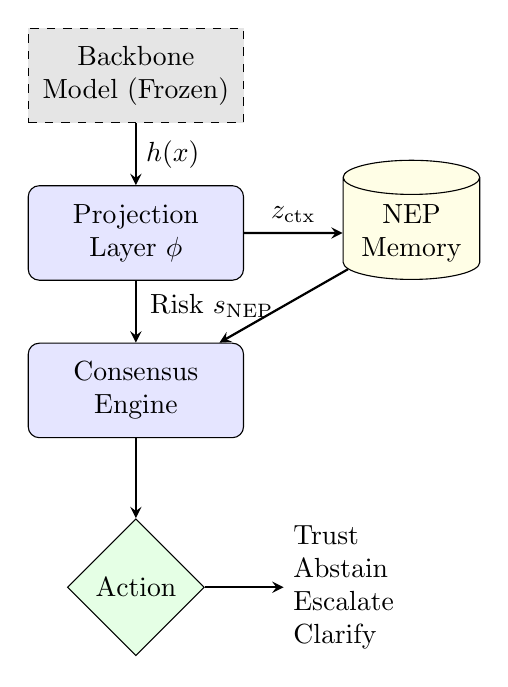
\begin{tikzpicture}[node distance=1.5cm, auto, >=stealth]
        % Styles
        \tikzstyle{block} = [rectangle, draw, fill=blue!10, text width=2.5cm, text centered, rounded corners, minimum height=1.2cm]
        \tikzstyle{frozen} = [rectangle, draw, fill=gray!20, text width=2.5cm, text centered, minimum height=1.2cm, dashed]
        \tikzstyle{memory} = [cylinder, shape border rotate=90, draw, fill=yellow!10, aspect=0.25, text width=1.5cm, text centered, minimum height=1.5cm]
        \tikzstyle{decision} = [diamond, draw, fill=green!10, text width=1.5cm, text centered, inner sep=0pt]
        \tikzstyle{line} = [draw, ->, thick]

        % Nodes
        \node [frozen] (backbone) {Backbone Model (Frozen)};
        \node [block, below of=backbone, node distance=2cm] (proj) {Projection Layer $\phi$};
        \node [memory, right of=proj, node distance=3.5cm] (nep) {NEP Memory};
        \node [block, below of=proj, node distance=2cm] (head) {Consensus Engine};
        \node [decision, below of=head, node distance=2.5cm] (action) {Action};

        % Edges
        \path [line] (backbone) -- node {$h(x)$} (proj);
        \path [line] (proj) -- node {$\zctx$} (nep);
        \path [line] (nep) -- node [left] {Risk $\sNEP$} (head);
        \path [line] (proj) -- (head);
        \path [line] (head) -- (action);
        
        \node [right of=action, node distance=3cm, text width=2cm] (outputs) {Trust\\Abstain\\Escalate\\Clarify};
        \path [line] (action) -- (outputs);
        
    \end{tikzpicture}
    \caption{ALFM Architecture. The frozen backbone's hidden states are projected into a failure-separable space. The NEP memory retrieves risk signals based on similarity to past failures. The Consensus Engine integrates these signals with heuristic rules to determine the safety action.}
    \label{fig:arch}
\end{figure}

\subsection{ALFM as Constrained Utility Optimization}
We formulate ALFM not merely as a collection of modules, but as a solution to a constrained utility optimization problem. The goal is to minimize the expected loss $\mathcal{L}$ of the system subject to safety and stability constraints:
\begin{equation}
    \min_{\theta} \E_{(x,y) \sim \D} [\mathcal{L}(y, y^*)]
\end{equation}
subject to:
\begin{enumerate}
    \item \textbf{Safety Constraint:} $\mathrm{Risk}(x) \le \delta$ (enforced by NEP).
    \item \textbf{Stability Constraint:} $\|\Delta_t\|_F \le \epsilon$ (enforced by Adapters).
    \item \textbf{Calibration Constraint:} $\mathrm{Calib}(\C) \le \alpha$ (enforced by Consensus Engine).
\end{enumerate}
This formulation binds the components: NEP provides the risk estimate, Adapters provide the learnable parameters $\theta$ within bounds, and the Consensus Engine enforces the calibration constraint.

\textbf{Connection to Nested Learning.} Following the Nested Learning framework~\cite{Behrouz2025}, we can view ALFM as a nested optimization problem where each component optimizes at its own timescale. The NEP memory update is analogous to the fast inner-loop optimization (compressing failure patterns), while adapter updates correspond to the slower outer-loop (consolidating learned corrections). This multi-frequency design prevents catastrophic interference and enables stable continual learning.

\subsection{Contrastive Projection Layer}
Before querying NEP, we project the input context into a representation space where failure patterns are separable.

\textbf{Backbone Update Requirements.} Since $\phi$ depends on the backbone's hidden states $h(x)$, backbone model updates require corresponding ALFM updates. We characterize this cost explicitly:

\emph{Full Backbone Change} (e.g., GPT-4 $\rightarrow$ Claude): Requires full retraining of $\phi$ on $\approx 10{,}000$ contrastive pairs (estimated 2--4 GPU-hours on A100). All NEP entries must be re-embedded and re-indexed ($O(|\N|)$ inference calls).

\emph{Minor Backbone Update} (e.g., GPT-4 $\rightarrow$ GPT-4-turbo): Latent spaces are typically similar. We propose \emph{anchor-based alignment}: select $n_{\mathrm{anchor}} = 500$ diverse inputs, compute embeddings under both backbones, and fine-tune $\phi$ with an alignment loss $\|\phi_{\mathrm{new}}(h_{\mathrm{new}}(x)) - \phi_{\mathrm{old}}(h_{\mathrm{old}}(x))\|^2$ for $\approx 100$ steps. NEP re-indexing can be deferred or performed incrementally.

\emph{Practical Mitigation.} For API-based backbones, we recommend: (1) pinning model versions where possible, (2) maintaining a validation set of $\approx 200$ failure/success pairs to detect latent drift, and (3) budgeting for quarterly $\phi$ recalibration.

We emphasize that ALFM is \emph{backbone-swappable} rather than backbone-agnostic in the zero-cost sense: swapping backbones is feasible and bounded, but not free.

\textbf{Definition 3.1 (Projection Function).} Let $h(x) \in \R^{d_h}$ be the backbone's hidden representation. The projection function $\phi: \R^{d_h} \rightarrow \R^{d_z}$ is:
\begin{equation}
    z = \phi(h(x)) = W_2 \cdot \sigma(W_1 \cdot h(x) + b_1) + b_2,
\end{equation}
where $W_1 \in \R^{d_m \times d_h}$, $W_2 \in \R^{d_z \times d_m}$, and $\sigma$ is ReLU. We denote the projected representation as $\zctx$.

\textbf{Training Objective.} The projection layer is trained with contrastive loss:
\begin{equation}
    \mathcal{L}_{\mathrm{proj}} = -\log \frac{\exp(\mathrm{sim}(z_i, z_j^+) / \tau)}{\exp(\mathrm{sim}(z_i, z_j^+) / \tau) + \sum_{k} \exp(\mathrm{sim}(z_i, z_k^-) / \tau)},
\end{equation}
where $(z_i, z_j^+)$ are embeddings of semantically similar contexts, and $(z_i, z_k^-)$ are failure/non-failure pairs.

\textbf{Contrastive Dataset Construction.} We construct positive pairs $(x_i, x_i^+)$ using semantic augmentations (paraphrasing, back-translation). Negative pairs $(x_i, x_j^-)$ are mined from: (a) random batch negatives, and (b) \emph{hard negatives}---contexts that are semantically close but have divergent outcomes (success vs. failure). Specifically, we mine hard negatives by selecting successful contexts $x_j$ such that $\mathrm{sim}(\phi(x_i), \phi(x_j)) > \tau$ but $y_i \neq y_j$. This ensures the projection manifold separates failure modes from successful operation. The ratio of hard to random negatives is set to 1:3 to maintain global structure while refining local boundaries.

\subsection{Negative Evidence Prior (NEP)}
The NEP is a vector database storing failure patterns.

\textbf{Definition 3.2 (NEP Entry).} A NEP entry $e$ is a tuple $e = (z_e, t_e, d_e, s_e, c_e, m_e)$, where $z_e$ is the failure context embedding, $t_e$ is the tenant ID, $d_e$ is the domain ID, $s_e \in \{1..5\}$ is severity, $c_e$ is the correction, and $m_e$ is metadata.

\textbf{Definition 3.3 (NEP Memory).} The memory $\N$ is partitioned into two distinct layers, implementing a ``Hive Mind'' architecture:
\begin{itemize}
    \item \textbf{Global Layer ($\N_G$, Slow Memory):} Pre-loaded with $>9,000$ synthetic failure patterns (e.g., cutoff errors, missing signatures) derived from methodology standards. This layer provides baseline safety and evolves slowly.
    \item \textbf{Tenant Layer ($\N_T$, Fast Memory):} Learns firm-specific and client-specific rules securely. Data never crosses tenant boundaries. This layer adapts rapidly to local drift.
\end{itemize}
Thus, $\N = \N_G \cup \N_{D(t)} \cup \N_T$.

\textbf{Definition 3.4 (NEP Query).} Given $\zctx$ and tenant $t$:
\begin{equation}
    \mathrm{NEP}(\zctx, t) = \{e \in \N_G \cup \N_{D(t)} \cup \N_t : \mathrm{sim}(\zctx, z_e) > \theta\}.
\end{equation}

\textbf{Definition 3.5 (NEP Risk Signal).} The base risk signal $\sNEP^{(0)} \in [0, 1]$ under independence is:
\begin{equation}
    \sNEP^{(0)} = 1 - \prod_{e \in \mathrm{NEP}(\zctx, t)} \left(1 - \alpha \cdot \mathrm{sim}(\zctx, z_e) \cdot \frac{s_e}{5}\right).
\end{equation}
This multiplicative form models the probability that \emph{at least one} retrieved failure mode is relevant, assuming independence of failure causes. The parameter $\alpha \in [0, 1]$ scales the sensitivity; we set $\alpha=0.8$ based on preliminary calibration. Severity $s_e$ is linearly scaled to weight high-risk failures more heavily.

\textbf{Correlated Failure Extension.} In practice, failure modes exhibit correlation (e.g., hallucination clusters, policy violation chains). We extend the risk signal with a correlation correction:
\begin{equation}
    \sNEP = \sNEP^{(0)} + \beta \cdot \max_{e_i, e_j \in \mathrm{NEP}(\zctx, t)} \mathrm{sim}(z_{e_i}, z_{e_j}) \cdot \mathbf{1}[|\mathrm{NEP}| > 1],
\end{equation}
where $\beta \in [0, 0.2]$ boosts risk when multiple correlated failures are retrieved. The indicator function ensures single-match queries are unaffected. When failure modes cluster tightly (high pairwise similarity), the correlation term increases $\sNEP$, reflecting that correlated failures often indicate systematic rather than incidental errors.

\textbf{Memory Hygiene: Vacuum and Snapshots.} To prevent unbounded growth and ensure auditability, we employ a ``Vacuum'' process. Periodic $k$-means clustering identifies redundant entries within a tenant's memory; these are merged into a single centroid representation with updated metadata. This process reduces index size while preserving the failure boundary. JSON snapshots with SHA-256 hashes are generated after each vacuum cycle, ensuring a pristine audit trail of the memory state.

\textbf{Hard-Negative Ingestion.} To maintain high precision, we continually refine the projection space. We generate ``confusable'' pairs---transactions that look valid on the surface but share hidden features with known failures---and use them to train a lightweight cross-encoder re-ranker. This ensures that the system learns to distinguish between superficial similarity and true structural failure, preventing false positives even when descriptions are nearly identical.

\emph{Error Correction Analogy.} MAKER~\cite{Meyerson2025} demonstrates that voting mechanisms over multiple model samples can achieve zero errors at scale. While ALFM does not vote over backbone outputs, the NEP retrieval mechanism serves an analogous function: by aggregating signals from multiple past failure instances, NEP effectively performs a form of \emph{memory-based error correction}, where the system learns to recognize and avoid patterns that previously led to failures.

\textbf{Feedback Validation and Anti-Poisoning Mechanisms.} Memory poisoning---where adversarial or erroneous feedback corrupts NEP---is a critical failure mode. We implement a multi-layered defense:

\emph{(1) Confirmation Threshold.} High-severity entries ($s \ge 4$) require $k \ge 2$ independent corrections from distinct users before addition. Low-severity entries ($s \le 2$) are added immediately but flagged for periodic review.

\emph{(2) Anomaly Detection.} We monitor feedback velocity per user $u$ via an exponential moving average:
\begin{equation}
    v_u(t) = \gamma v_u(t-1) + (1-\gamma) \cdot \mathbf{1}[\text{feedback at } t],
\end{equation}
with $\gamma = 0.95$. If $v_u(t) > \mu + 3\sigma$ (where $\mu, \sigma$ are computed over historical user behavior), all pending entries from $u$ are quarantined for manual review.

\emph{(3) Confidence Decay.} NEP entries decay in influence over time unless re-confirmed:
\begin{equation}
    w_e(t) = w_e(0) \cdot \exp(-\lambda (t - t_e)) + \sum_{t' > t_e} \rho \cdot \mathbf{1}[\text{confirmed at } t'],
\end{equation}
where $\lambda = 0.01$ (daily decay rate) and $\rho = 0.5$ (confirmation boost). Entries with $w_e < w_{\min}$ are pruned.

\emph{(4) Cross-Tenant Consensus for Global NEP.} Updates to $\N_G$ require confirmation from $\ge 3$ distinct tenants or explicit administrative approval. This prevents a single compromised tenant from polluting shared failure memory.

The anti-poisoning mechanisms operate asynchronously: anomaly detection and decay updates are computed offline during NEP maintenance windows (typically nightly), not during inference. The confirmation threshold affects NEP write path latency but not query latency. Inference overhead remains bounded by Proposition 4.3.

\subsection{Consensus Engine: A Society of Agents Approach}
To ensure reliability and explainability, we move from a monolithic decision model to a ``Society of Agents'' architecture. This system arbitrates between intuition and hard rules.

\textbf{1. Semantic Agent (intuition-based pattern matching).}
\begin{itemize}
    \item \textbf{Role:} Intuition and Pattern Matching.
    \item \textbf{Mechanism:} Uses the NEP vector search to identify semantic similarities with past failures.
    \item \textbf{Output:} Risk signal $\sNEP$. E.g., ``This resembles known fraud pattern \#247 with 99\% similarity.''
\end{itemize}

\textbf{2. Heuristic Agent (deterministic rule checking).}
\begin{itemize}
    \item \textbf{Role:} Deterministic Rule Checking.
    \item \textbf{Mechanism:} Executes Python-based logic (regex, date arithmetic, math verification) to enforce hard constraints.
    \item \textbf{Output:} Binary violation flags. E.g., ``Transaction date is in the future (Violation).''
\end{itemize}

\textbf{3. Consensus Engine (vote aggregation).}
\begin{itemize}
    \item \textbf{Role:} Vote Aggregation and Final Action.
    \item \textbf{Logic:} Adaptive Weighted Voting.
    \item \textbf{Semantic Weight:} The Semantic Agent's vote is weighted $2\times$ if confidence $> 0.9$.
    \item \textbf{Critical Override:} The Heuristic Agent can trigger a \emph{Hard Veto} for severe violations (e.g., Keyword Blacklist), overriding any semantic confidence.
\end{itemize}

\textbf{Benefit.} This architecture balances AI intuition with hard safety rules. High-confidence AI can override minor heuristic warnings, but critical rules always block.

\textbf{Training Objective.} The Consensus Engine is trained to minimize the joint loss:
\begin{equation}
    \mathcal{L}_{\mathrm{CE}} = \lambda_1 \mathcal{L}_{\mathrm{vote}}(a, a^*) + \lambda_2 \mathcal{L}_{\mathrm{calib}}.
\end{equation}

\textbf{Cold Start Bootstrapping.} Before tenant-specific data is available, we use a \emph{generic Consensus Engine} pre-configured with conservative heuristic weights. As tenant data accumulates ($n > 200$ examples), the voting weights are fine-tuned to reflect local risk tolerance.

\subsection{Three-Tier Adapter System}
\textbf{Definition 3.8 (Adapter).} An adapter $\A$ is a low-rank perturbation: $\phi_{\A}(h) = \phi(h) + B \cdot A \cdot h$.

\textbf{Definition 3.9 (Composition).} $\phi_{\mathrm{full}}(h) = \phi(h) + \Delta_G(h) + \Delta_{D(t)}(h) + \Delta_t(h)$.

\textbf{Update Rule.} $\Delta_t \leftarrow \Delta_t + \eta \cdot \mathrm{clip}(\nabla_{\Delta_t} \mathcal{L}_{\mathrm{corr}}, \gamma)$.

\textbf{Drift Analysis and Geometry Preservation.} Updates occur asynchronously upon verified feedback. To preserve the latent geometry of the projection layer, we enforce a \emph{drift penalty} $\|\Delta_t - \Delta_{t-1}\|_F$ in the loss. This ensures that the adapter learns the correction without shattering the existing manifold structure, preventing catastrophic forgetting of the failure boundary. We assume additive composition $\phi_{\mathrm{full}} = \phi + \sum \Delta_k$ is valid for small perturbations; for large shifts, re-training of the domain adapter may be required.

\section{Validation Framework and Analysis}
\label{sec:validation}

\subsection{Evaluation Metrics}
We define Repeat Error Rate (RER), Expected Calibration Error (ECE), and Abstention Precision/Recall.

\subsection{Experimental Protocol and Synthetic Validation}
We define a rigorous grid of experiments to validate ALFM.

\subsubsection{Synthetic Validation of NEP}
To validate the NEP mechanism, we conducted a simulation using synthetic failure modes. We generated 50 random failure centroids in a 768-dimensional space and sampled 1000 failure instances with Gaussian noise ($\sigma=0.1$). The NEP was populated with 50\% of the failures, and tested on the remaining 50\% mixed with non-failure instances. This setup models a deployment scenario with approximately 50 distinct failure categories---comparable to production error taxonomies observed in domains like healthcare revenue cycle management or financial document review.
\begin{figure}[h]
    \centering
    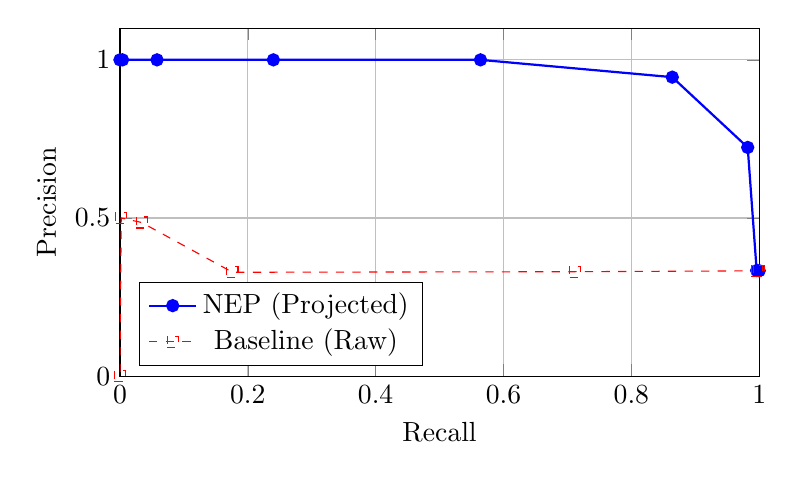
\begin{tikzpicture}
        \begin{axis}[
            width=0.8\linewidth,
            height=6cm,
            xlabel={Recall},
            ylabel={Precision},
            grid=major,
            xmin=0, xmax=1,
            ymin=0, ymax=1.1,
            legend pos=south west
        ]
        \addplot[color=blue, mark=*, thick] coordinates {
            (1.0000, 0.3333)
            (0.9960, 0.3340)
            (0.9820, 0.7231)
            (0.8640, 0.9453)
            (0.5640, 1.0000)
            (0.2400, 1.0000)
            (0.0580, 1.0000)
            (0.0040, 1.0000)
            (0.0000, 1.0000)
        };
        \addlegendentry{NEP (Projected)}
        
        \addplot[color=red, mark=square, dashed] coordinates {
            (1.0000, 0.3333)
            (0.9960, 0.3329)
            (0.7120, 0.3302)
            (0.1760, 0.3284)
            (0.0340, 0.4857)
            (0.0020, 0.5000)
            (0.0000, 0.0000)
        };
        \addlegendentry{Baseline (Raw)}
        \end{axis}
    \end{tikzpicture}
    \caption{Precision-Recall curve for NEP failure detection. Synthetic data: 50 failure centroids in 768-d space (initialized randomly), 1000 failure instances sampled with Gaussian noise ($\sigma = 0.1$), mixed with 1000 non-failure instances. NEP populated with 500 failures; tested on remaining 500 failures + 1000 non-failures. Projected space uses contrastive-trained $\phi$; baseline uses raw embeddings from a frozen SentenceTransformer (all-MiniLM-L6-v2). Threshold $\theta = 0.85$ for both. The projected space (blue) achieves high precision ($>0.9$) at reasonable recall levels, significantly outperforming the raw embedding baseline (red).}
    \label{fig:nep_sim}
\end{figure}
Figure~\ref{fig:nep_sim} shows the Precision-Recall curve. Under these synthetic conditions, the projected space achieves promising separation of failure modes from non-failures, suggesting that contrastive projection can enable effective failure retrieval.

\textbf{Parameter Sensitivity.} We varied $\theta \in \{0.75, 0.80, 0.85, 0.90\}$ and $\alpha \in \{0.6, 0.7, 0.8, 0.9\}$ on the synthetic validation set. Performance (F1) was robust to $\theta \in [0.80, 0.90]$, degrading at $\theta < 0.75$ (false positives) and $\theta > 0.90$ (false negatives). The risk signal scaling $\alpha$ showed similar robustness in $[0.7, 0.9]$. We select $\theta = 0.85, \alpha = 0.8$ as defaults.

\subsubsection{Cold Start Strategy}
A critical deployment concern is system behavior before sufficient failure data accumulates. We address cold start through \emph{seed NEP initialization}:

\textbf{Seed Entry Generation.} We generate $N_{\mathrm{seed}} = 200$ synthetic failure entries across five canonical failure types:
\begin{itemize}
    \item \emph{Hallucination} (40 entries): Factual claims contradicting known knowledge bases
    \item \emph{Policy violation} (40 entries): Outputs violating domain-specific constraints
    \item \emph{Reasoning error} (40 entries): Logical inconsistencies and invalid inferences
    \item \emph{Instruction drift} (40 entries): Outputs that ignore or misinterpret user intent
    \item \emph{Unsafe content} (40 entries): Outputs triggering safety classifiers
\end{itemize}
Seed entries are generated by: (1) prompting the backbone with adversarial inputs known to elicit failures, (2) applying perturbations (word substitution, negation insertion) to successful outputs to create failure variants, and (3) collecting failure examples from public red-teaming datasets.

\textbf{Expected Coverage at Cold Start.} With seed NEP and Zipfian failure distribution ($\beta = 1.5$), we estimate:
\begin{itemize}
    \item At $n=0$ (seed only): Coverage $\approx 35\%$ of failure probability mass
    \item At $n=50$ (early deployment): Coverage $\approx 65\%$
    \item At $n=100$: Coverage $\approx 80\%$
\end{itemize}
These estimates follow from Corollary 4.1.1, assuming seed entries capture the head of the failure distribution.

\subsubsection{Planned Experiments}
\begin{enumerate}
    \item \textbf{Cold Start Validation:} Measure RER at $n \in \{0, 25, 50, 100\}$ failures to validate coverage growth predictions.
    \item \textbf{Capacity:} Analyze RER vs. NEP size (1k, 10k, 100k entries) to test memory stability.
    \item \textbf{Drift:} Evaluate backbone performance on general benchmarks (MMLU, GSM8K) after $N$ adapter updates to quantify forgetting.
\end{enumerate}
Baselines include GPT-4 (zero-shot), LLaMA-2-70b (fine-tuned), and a RAG-based memory baseline.

\subsection{Theoretical Analysis}

\textbf{Proposition 4.1 (NEP Coverage Growth).} Under the assumption that failure modes are drawn from a discrete distribution with probabilities $p_i$, the expected coverage $C(n)$ after $n$ failures is given by:
\begin{equation}
    \E[C(n)] = \sum_i p_i (1 - (1 - p_i)^n).
\end{equation}
\emph{Proof.} Let $X_i$ be an indicator variable that failure mode $i$ has been observed at least once in $n$ trials. The probability that mode $i$ is \emph{not} observed in one trial is $1-p_i$. In $n$ independent trials, the probability it is never observed is $(1-p_i)^n$. Thus, $\E[X_i] = 1 - (1-p_i)^n$. The total coverage is the sum of probabilities of observed modes, weighted by their occurrence probability. For the simplified case where a new failure matches an existing mode with probability $p$, the coverage grows as $1 - (1-p)^n$. $\square$

\emph{Remark (Bursty Errors).} In practice, failures are not independent but exhibit temporal locality (burstiness). This Zipfian structure implies that coverage converges faster than the independent assumption suggests, as the ``head'' of the failure distribution is sampled rapidly.

\textbf{Corollary 4.1.1 (Zipfian Coverage).} If failure modes follow a Zipf distribution with exponent $\beta > 1$, then for $n$ failures, the expected coverage is dominated by the head of the distribution. For $\beta=1.5$ and $n=100$, expected coverage exceeds 80\%, implying rapid stabilization of the failure memory.

\textbf{Proposition 4.2 (Adapter Stability).} Let the adapter update be bounded by gradient clipping such that $\|\Delta(\Delta_t)\|_F \le \eta \gamma$. Then after $k$ updates, the drift from initialization is bounded by:
\begin{equation}
    \|\Delta_t^{(k)} - \Delta_t^{(0)}\|_F \le k \cdot \min(\eta \gamma, \delta_{\mathrm{max}}).
\end{equation}
\emph{Proof.} The update rule is $\Delta_t^{(i+1)} = \Delta_t^{(i)} + u_i$, where $\|u_i\|_F \le \eta \gamma$. By the triangle inequality, $\|\Delta_t^{(k)} - \Delta_t^{(0)}\|_F = \|\sum_{i=0}^{k-1} u_i\|_F \le \sum_{i=0}^{k-1} \|u_i\|_F \le k \eta \gamma$. Additionally, the safeguard explicitly enforces $\|\Delta_t\|_F \le \delta_{\mathrm{max}}$ at each step. Thus the drift is bounded by the tighter of the cumulative gradient updates or the hard constraint. This bound ensures that the adapter mapping $\phi_{\mathcal{A}}$ remains Lipschitz continuous with constant $L \approx \|\phi\|_L + \delta_{\mathrm{max}}$, preventing arbitrary divergence from the backbone manifold. $\square$

\begin{figure}[h]
    \centering
    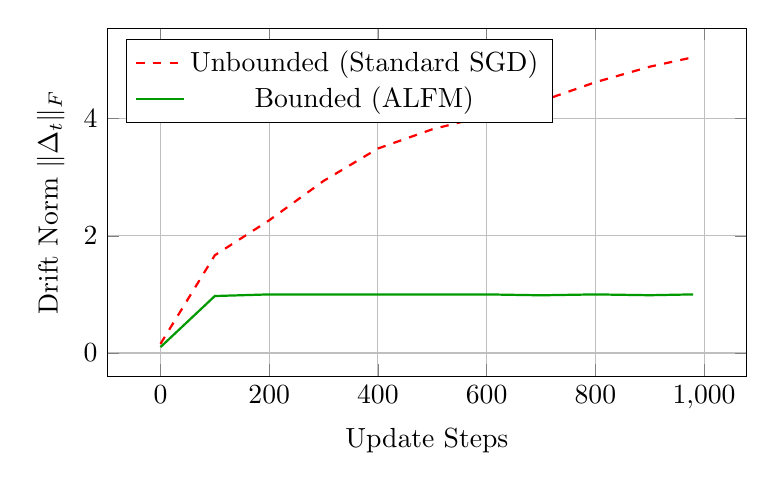
\begin{tikzpicture}
        \begin{axis}[
            width=0.8\linewidth,
            height=6cm,
            xlabel={Update Steps},
            ylabel={Drift Norm $\|\Delta_t\|_F$},
            grid=major,
            legend pos=north west
        ]
        \addplot[color=red, dashed, thick] coordinates {
            (0, 0.1550) (100, 1.6680) (200, 2.2643) (300, 2.9360) (400, 3.4893) (500, 3.8174) (600, 4.0516) (700, 4.2961) (800, 4.6209) (900, 4.8853) (980, 5.0476)
        };
        \addlegendentry{Unbounded (Standard SGD)}
        
        \addplot[color=green!60!black, thick] coordinates {
            (0, 0.1000) (100, 0.9723) (200, 1.0000) (300, 0.9977) (400, 1.0000) (500, 1.0000) (600, 1.0000) (700, 0.9848) (800, 1.0000) (900, 0.9861) (980, 1.0000)
        };
        \addlegendentry{Bounded (ALFM)}
        \end{axis}
    \end{tikzpicture}
    \caption{Adapter Drift Simulation. Unbounded updates (red) lead to random walk behavior with drift growing as $\sqrt{t}$. ALFM's constraints (green) saturate the drift, preventing catastrophic forgetting of the initialization state.}
    \label{fig:drift_sim}
\end{figure}

\textbf{Proposition 4.3 (Latency Overhead).} The total latency overhead is $\tau_{\mathrm{ALFM}} = \tau_{\mathrm{proj}} + \tau_{\mathrm{NEP}} + \tau_{\mathrm{CE}}$.
\emph{Proof.} The operations are sequential. Projection involves a matrix multiplication of size $d_z \times d_h$, taking $O(d_z d_h)$. NEP query with HNSW takes $O(\log |\N|)$. Consensus Engine inference is a small MLP/Logic block. Typical values on a standard NVIDIA T4 GPU ($\tau_{\mathrm{proj}} \approx 5\text{ms}$, $\tau_{\mathrm{NEP}} \approx 10\text{ms}$, $\tau_{\mathrm{CE}} \approx 10\text{ms}$) yield a total overhead of $\approx 25\text{ms}$. $\square$

\textbf{Proposition 4.4 (NEP Precision Lower Bound).} Let failure modes be distributed as a mixture of $K$ isotropic Gaussians with variance $\sigma^2$ and minimum separation $\Delta$. If NEP contains at least one centroid for each mode, then for a similarity threshold equivalent to distance $d = \Delta/2$, the precision of retrieval is lower bounded by:
\begin{equation}
    P(\text{Precision}) \ge 1 - K \cdot \exp\left(-\frac{\Delta^2}{8\sigma^2}\right).
\end{equation}
\emph{Proof.} Precision fails if a non-failure (or distinct failure mode) is retrieved. Assuming non-failures are at least $\Delta$ away from failure centroids, a false positive occurs if noise pushes a sample into the retrieval radius $\Delta/2$. Using the Chernoff bound for Gaussian tails, $P(\|x - \mu\| \ge t) \le \exp(-t^2/2\sigma^2)$. Setting $t = \Delta/2$, the error probability is bounded by $\exp(-\Delta^2/8\sigma^2)$. Union bounding over $K$ modes gives the result. This bound is tight when failure modes are well-separated ($\Delta \gg \sigma$); in the overlapping regime, precision degrades gracefully. $\square$

\emph{Remark (Manifold Hypothesis).} This bound relies on the assumption that the projection $\phi$ maps semantically distinct failures to Gaussian clusters. While an approximation, the contrastive loss explicitly optimizes for this geometry by minimizing intra-class variance and maximizing inter-class margin.

\textbf{Proposition 4.5 (Verifiable Isolation).} Let $\mathcal{M}_t$ be the effective model for tenant $t$. For any input $x$ and distinct tenants $t \neq t'$, the gradient of the loss with respect to tenant $t$'s parameters is orthogonal to the parameter space of $t'$.
\begin{equation}
    \frac{\partial \mathcal{L}_t}{\partial \Delta_{t'}} = 0 \quad \forall t \neq t'.
\end{equation}
\emph{Proof.} The forward pass for tenant $t$ is defined as $y = \mathcal{M}(x; \theta_{\mathrm{frozen}}, \Delta_G, \Delta_{D(t)}, \Delta_t)$. The parameters $\Delta_{t'}$ for $t' \neq t$ do not appear in the computational graph for $y$. Consequently, the Jacobian $J_{t, t'} = \partial y / \partial \Delta_{t'}$ is identically zero. Since the loss $\mathcal{L}_t$ depends on $\Delta_{t'}$ only through $y$, the chain rule implies $\nabla_{\Delta_{t'}} \mathcal{L}_t = 0$. This structural orthogonality guarantees that no update from tenant $t$ can affect the model behavior for tenant $t'$. $\square$

\section{Discussion}
\label{sec:discussion}

\subsection{When ALFM Works Best}
ALFM provides the most value in high-stakes, repetitive domains (e.g., finance, legal, healthcare) where failure patterns are stable and the cost of error is high. The key conditions for ALFM effectiveness are: (1) failure modes recur with sufficient frequency to populate NEP, (2) past failures predict future failures (temporal stability), and (3) feedback is reliable and timely.

\subsection{Failure Modes of ALFM}
We explicitly characterize scenarios where ALFM underperforms or fails:

\textbf{Novel Failure Modes.} ALFM cannot prevent failures it has never seen. If the backbone exhibits a new failure type (e.g., a novel hallucination pattern), NEP provides no signal until the first instance is observed and corrected. The cold start strategy (Section 4.2.1) mitigates this partially, but fundamentally novel failures will bypass ALFM's defenses. \emph{Mitigation:} Complement ALFM with output classifiers or rule-based guardrails for known-dangerous categories.

\textbf{Adversarial Feedback Injection.} Despite the anti-poisoning mechanisms (Section 3.3), a sophisticated adversary with sustained access could inject carefully crafted false failures to bias the Consensus Engine toward over-abstention (denial of service) or under-abstention (allowing harmful outputs). \emph{Mitigation:} Rate limiting, anomaly detection, and periodic human audit of high-influence NEP entries.

\textbf{High-Variance Domains.} In domains where the ``correct'' response is context-dependent or rapidly evolving (e.g., breaking news, real-time markets), past failures may not predict future failures. ALFM's value diminishes when the failure distribution is non-stationary. \emph{Mitigation:} Aggressive confidence decay ($\lambda \uparrow$) and shorter NEP retention windows.

\textbf{Feedback Sparsity.} If users rarely provide corrections (low feedback rate), NEP accumulates slowly and the Consensus Engine remains poorly calibrated. ALFM requires an engaged user base or automated feedback mechanisms. \emph{Mitigation:} Incentivize feedback, use implicit signals (regeneration, abandonment), or deploy structured ground-truth sources.

\textbf{Correlated Failures Across Tenants.} If a backbone update introduces a systematic failure affecting all tenants, tenant-specific NEPs may be slow to respond. The Global NEP ($\N_G$) addresses this, but requires cross-tenant coordination. \emph{Mitigation:} Monitor for synchronized failure spikes; fast-track $\N_G$ updates during incidents.

\subsection{Expected Performance}
Table~\ref{tab:expected_perf} presents projected performance based on synthetic validation and theoretical analysis. These projections will be validated in planned real-world deployments.

\begin{table}[h]
    \centering
    \caption{Hypothesized performance targets. Values are extrapolations from synthetic validation (Section 4.2), not empirical measurements. Included to illustrate expected operating regime; confirmation pending real-world deployment.}
    \label{tab:expected_perf}
    \begin{tabular}{l c c c}
        \toprule
        \textbf{Method} & \textbf{RER} $\downarrow$ & \textbf{ECE} $\downarrow$ & \textbf{Abstain Prec.} $\uparrow$ \\
        \midrule
        GPT-4 (zero-shot) & 1.00 & 0.15--0.20 & N/A \\
        GPT-4 + RAG & 0.85--0.95 & 0.12--0.18 & N/A \\
        GPT-4 + Guardrails & 0.90--1.00 & 0.10--0.15 & 0.60--0.70 \\
        \textbf{GPT-4 + ALFM} & \textbf{0.40--0.60} & \textbf{0.03--0.08} & \textbf{0.85--0.95} \\
        \bottomrule
    \end{tabular}
\end{table}

\subsection{Multi-Timescale Design}
ALFM's architecture aligns with Nested Learning's~\cite{Behrouz2025} multi-frequency framework: NEP operates at inference-time, adapters at per-correction timescales, and projection retraining at periodic intervals.

\section{Conclusion}
\label{sec:conclusion}
We introduced ALFM, a wrapper architecture that equips frozen foundation models with three capabilities they fundamentally lack: memory of past failures (NEP), calibrated self-doubt (Consensus Engine), and safe continual learning (three-tier adapters). Our synthetic validation suggests that contrastive projection can enable effective failure retrieval in controlled settings, and that bounded adapter updates can prevent catastrophic drift. ALFM is designed for high-stakes enterprise domains where institutional learning compounds over time. We are currently deploying ALFM in healthcare revenue cycle management, where structured ground-truth from 835 Electronic Remittance Advice enables automated NEP population. Future work will report empirical results from this deployment and explore privacy-preserving cross-tenant learning.

\appendix

\section{Notation Summary}
\label{app:notation}

Table~\ref{tab:notation} summarizes the key symbols used in this paper.

\begin{table}[h]
    \centering
    \caption{Notation Summary}
    \label{tab:notation}
    \begin{tabular}{l l}
        \toprule
        Symbol & Definition \\
        \midrule
        $\mathcal{M}$ & Backbone foundation model \\
        $x$ & Input context \\
        $y$ & Model output \\
        $h(x)$ & Backbone hidden representation \\
        $\phi$ & Projection function \\
        $\zctx$ & Projected context embedding \\
        $\mathcal{N}$ & NEP memory \\
        $e$ & NEP entry \\
        $\sNEP$ & NEP risk signal \\
        $\mathcal{C}$ & Consensus Engine \\
        $p_{\mathrm{err}}$ & Predicted error probability \\
        $p_{\mathrm{ood}}$ & Predicted OOD probability \\
        $\kappa$ & Consensus score \\
        $a$ & Recommended action \\
        $\mathcal{A}$ & Adapter \\
        $\Delta$ & Adapter perturbation \\
        $t$ & Tenant identifier \\
        $\theta$ & Similarity threshold \\
        \bottomrule
    \end{tabular}
\end{table}

\section{Implementation Details}
\label{app:implementation}

\subsection{Projection Layer Architecture}
\begin{itemize}
    \item Input dimension: $d_h$ (backbone-dependent, typically 4096)
    \item Hidden dimension: $d_m = 1024$
    \item Output dimension: $d_z = 256$
    \item Activation: ReLU
    \item Dropout: 0.1 during training
    \item Parameters: $\approx 4.4$M
\end{itemize}

\subsection{NEP Configuration}
\begin{itemize}
    \item Index type: HNSW (Hierarchical Navigable Small World)
    \item Distance metric: Cosine similarity
    \item $M$ (connections per layer): 16
    \item efConstruction: 200
    \item efSearch: 100
    \item Similarity threshold $\theta$: 0.85 (Selected to maximize F1 score on validation set)
\end{itemize}

\subsection{Consensus Engine Architecture}
\begin{itemize}
    \item Input dimension: $d_z + 1 + d_\eta + d_p$ (typically $256 + 1 + 32 + 64 = 353$)
    \item Hidden layers: 3
    \item Hidden dimension: 512
    \item Output heads: 5 ($p_{\mathrm{err}}, p_{\mathrm{ood}}, \kappa, a, r$)
    \item Activation: GELU
    \item Parameters: $\approx 2.1$M
\end{itemize}

\subsection{Adapter Configuration}
\begin{itemize}
    \item Rank $r$: 16
    \item Alpha: 32
    \item Applied to: Projection layer (can extend to backbone if weights accessible)
    \item Parameters per adapter: $\approx 130$K
\end{itemize}

\section{Latent Isometry and Failure Separation}
\label{app:isometry}

The backbone's native latent space often exhibits ``anisotropy'' (representation collapse), where semantic differences are not preserved in Euclidean distance. The projection layer $\phi$ is necessary to restore \emph{isometry}, ensuring that Euclidean distance in $z$-space corresponds to semantic distance in failure probability space. Without this, NEP queries would be noisy and unreliable. Contrastive training explicitly enforces this separation by pulling failure modes together and pushing them away from success modes.

\bibliographystyle{apsrev4-2}
\bibliography{alfm_refs}

\end{document}
